\scanpage{91}
% archive foliation: 90
Ainsi, on obtient via le pol. car. modifié un
hom
\[
(V,f)\longmapsto\frac1{\det(\mathrm{id}_V-ft)}=L(V,f)
\]
\[
R(\unsure{\mathbf N|\mathbf Z};k)\longrightarrow 1+k[[t]]^+
\]
\inserted{Composé avec l'\deleted{\unsure{isomorphisme|homomorphisme}}\inserted{aut° ``additif''}
$\varphi(t)\longmapsto\dfrac1{\varphi(t)}$ dans $1+k[[t]]^+$}
qui est un hom de $\lambda$-anneaux,
\margin{\figure{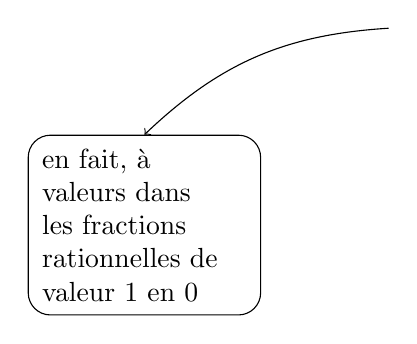
\begin{tikzpicture}[x=1cm,y=1cm]
\node[draw,rounded corners=8pt,align=left,text width=2.6cm,inner sep=5pt] (note) at (0,0) {en fait, à valeurs dans les \uline{fractions rationnelles} de valeur $1$ en $0$};
\draw[->] (3.1,2.5) to[bend right=20] (note.north);
\end{tikzpicture}}}

Lorsque $k$ est un corps, l'hom
précédent est injectif. En effet, si
\deleted{$k$ est \unsure{alg. clos},} la connaissance de la
série formelle permet de reconstituer \inserted{la fonction rationnelle}
[$k[t]$
étant factoriel] l'élément
$\displaystyle\sum_{\substack{P\ \unsure{pol.|irr.}\\\mathrm{unitaires}}}c_P(V_P,f_P)$
\deleted{dont} par
\[
L=\prod_Q Q^{c_P}
\]
[$Q$ et $P$ associés de
la façon précisée plus haut].

Notons qu'on a un homomorphisme
naturel \deleted{\unsure{$k$ séparé alg.}}
\[
1+k[[t]]^+\longrightarrow k[[t]]
\]
\[
\varphi(t)\longmapsto\frac{\varphi'(t)}{\varphi(t)}\deleted{\unsure{t}}
\]
qui correspond à
\[
\Lambda(V,f)(t)=\frac{L(V,f)'(t)}{L(V,f)(t)}
=[\log L(V,f)]'=\frac1t\sum_1^\infty(\operatorname{Tr}f^n)t^n.
\]
\deleted{En car. $0$, on peut}
Si $k$ de car. $0$, \inserted{i.e. $k\supset\mathbf Q$} on peut inverser cet
homomorphisme par $\exp\left(\int_0^{\unsure{t}}\Lambda(V,f)(t)\right)$.
Donc \inserted{si $k$ est \margin{un corps de car. $0$,}}
$\Lambda:R(\mathbf N,k)\longrightarrow k[[t]]$ est aussi injectif \deleted{($k$ corps}
